% Chapter 3

\chapter{DESIGN AND ARCHITECTURE}

% \begin{figure}[hbt] 
% \begin{center}
% \includegraphics[scale=.40]{./figures/bddig1}
% \caption{\label{fig:BDDD}A BDD where some boolean variables occur more than
% once on an evaluation path.}
% \end{center}
% \end{figure}

We propose a machine learning based student program evaluation system which represents student programs as a set of features extracted from the source programs and the AST representation of the source programs. Deep learning is purposely avoided since it would make the program's representation difficult to comprehend. The ML models are regression models which will output a score between 0 to 10 for each program submission. Feedback is provided to each program submission based on comparing the feature vector of the program with the average feature vector of 'good' programs.


\section{TRAINING} 

The dataset contains the code and corresponding scores for each of the
student programs. Features from code were extracted by using two
ways. Some features were extracted directly from the code. For the
other features, the code was first transformed into an Abstract Syntax
Tree(AST); then the features were extracted from the AST. The extracted
features were used to train the model. Three models were trained
separately: Linear Support vector regressor(SVR) , Random forest and Multi layer
perceptron(MLP) regressor. The models trained were all regression models which were
trained to predict the scores that should be given to the evaluated
codes.

\begin{figure}[h]
\centering
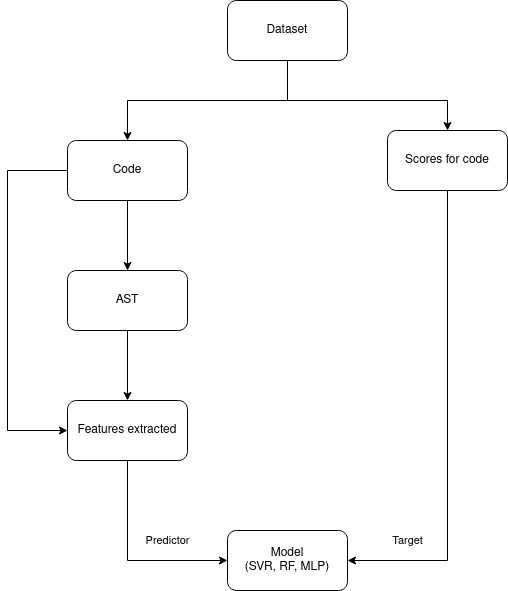
\includegraphics[width=0.9\textwidth]{./training.jpg}
\caption{Training}
\label{fig1}
\end{figure}

\newpage

\section{DEPLOYMENT} 

\begin{figure}[H]
\centering
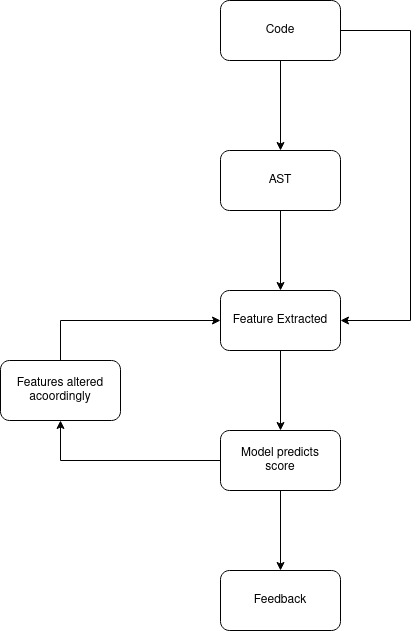
\includegraphics[scale=0.7]{./Deployment.jpg}
\caption{Deployment}
\label{fig1}
\end{figure}

The student code is the input. Features are extracted from the code as
explained in the section above. Some features are extracted from the
code itself and the rest from an AST representation of the code. This
feature set is input into the trained models from the previous
section. The model predicts a score for the input code based on the
feature set.

As explained earlier, our model is trained only with the feature values of the program and its score. Our trained model will evaluate how modifications in program's features can lead to a better score and thus there is no necessity for a explicitly annotated dataset with feedbacks for each code. 

From the training dataset, average feature vector $x$ is computed for the "excellent" programs(programs with a perfect score of 10). Feedback is generated with correspondence to the difference between the feature values of the submitted program and the average feature vector of the excellent programs.



\section{ALGORITHMS}

After representing code solutions as feature vectors, the dataset was
exported to perform training for machine learning models. The
following models
\begin{itemize}
    \item Support Vector Machine (SVM)
    \item Random Forest 
    \item Multi Layer Perceptron (MLP)
\end{itemize}
were employed for training. The detailed description of the mentioned
algorithms are listed below.

\section{SUPPORT VECTOR MACHINE}

Support Vector Machines (SVMs) are supervised learning models with associated learning algorithms that examine data for classification and regression in machine learning. Support Vector Regression \cite{D} is used to predict continuous values. The Support Vector Machine and Support Vector Regression are both based on the same premise (SVM). The goal of a support vector machine method is to find a hyperplane in an n-dimensional space that categorises data points clearly. Support Vectors are the data points on each side of the hyperplane that are closest to the hyperplane. These have an effect on the hyperplane's location and orientation, and so aid in the construction of the SVM.

\subsection{Hyperparameters in SVR}

Following are the various key hyper parameters used in Support Vector Regression.
\begin{figure}[h]
\centering
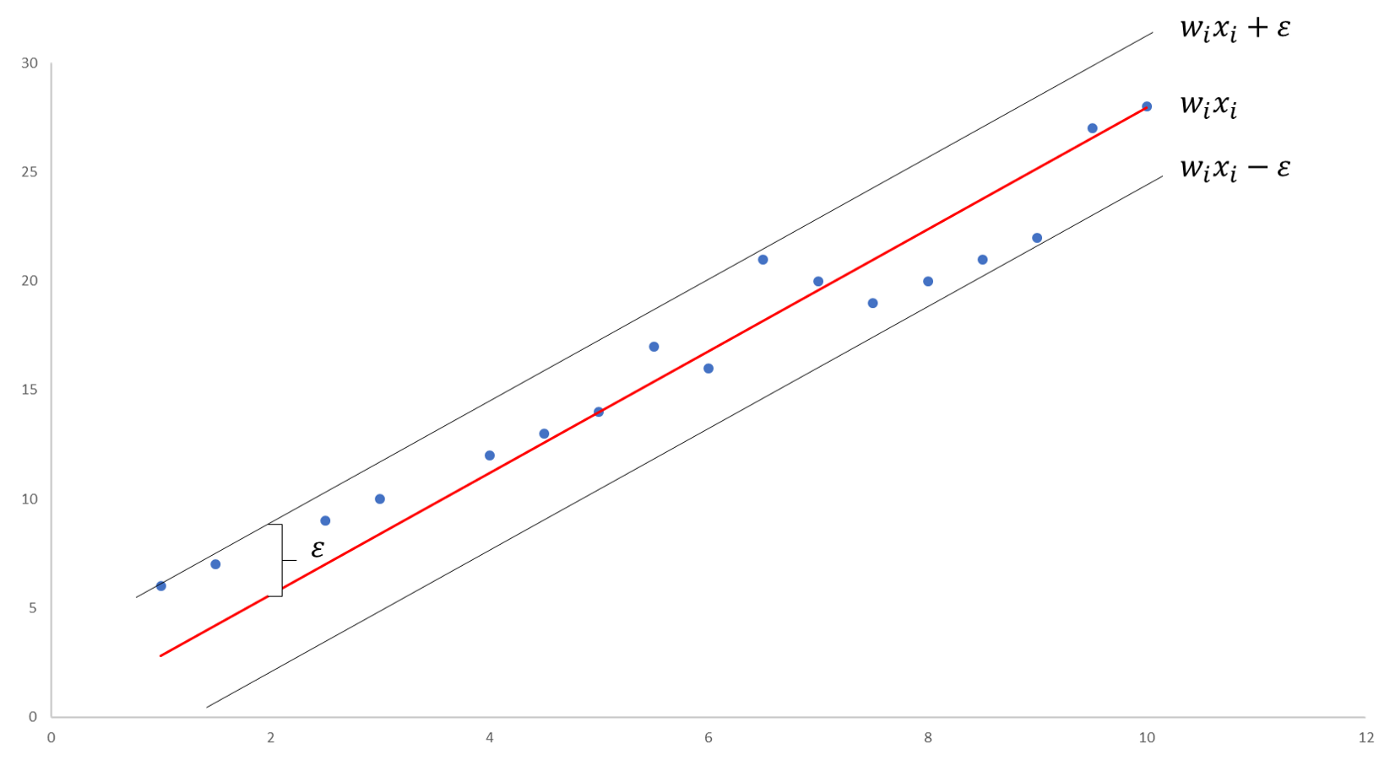
\includegraphics[width=1\textwidth, height=15cm]{./figures/svm.png}
\caption{Simple SVR}
\label{fig1}
\end{figure}

\begin{itemize}
\item \textbf{Hyperplane} (Red line in Figure~4.3) \\ A decision boundary that forecasts continuous output is known as a hyperplane. Support Vectors are the data points on each side of the hyperplane that are closest to the hyperplane. These are used to draw the essential line that depicts the algorithm's projected outcome.
\item \textbf{Kernel} \\ A kernel is a collection of mathematical functions that take input data and transform it into the required form. These are most commonly employed to locate a hyperplane in higher-dimensional space.
\item \textbf{Boundary Lines} (Grey lines in Figure~4.3) \\ 
These are the two lines that are drawn at an \textbf{$\epsilon$} (epsilon) distance around the hyperplane. It's used to separate the data points by a margin.

\end{itemize}

\subsection{Support Vector Regression}

The best fit line or hyperplane with the most points is found using Support Vector Regression (SVR). The SVR, unlike other regression models, aims to fit the best line within a threshold value, rather than minimising the error between the real and projected value (the distance between the hyperplane and boundary line). As a result, we'll only consider points that fall inside the decision boundary and have the lowest error rate, or those that fall within the margin of tolerance. This results in a more accurate model.

%\newpage

\section{RANDOM FOREST}

Random forest is a frequently used supervised machine learning algorithm for classification and regression tasks. The functioning of
Random Forest is contingent on three main factors,
\begin{itemize}
\item Decision Trees
\item Ensemble Learning
\item Bootstrapping
\end{itemize}

The following subsections % (6.2.1, 6.2.2 and 6.2.3)
detail on the mentioned factors description.

\subsection{Ensemble Learning}

Ensemble learning is the process of combining many models that have been trained on the same data and averaging their findings to provide a more accurate predictive/classification result. Ensemble learning requires that the errors of each model (a decision tree model) be independent and distinct from one another.

\subsection{Decision Tree}

\begin{figure}[h]
\centering
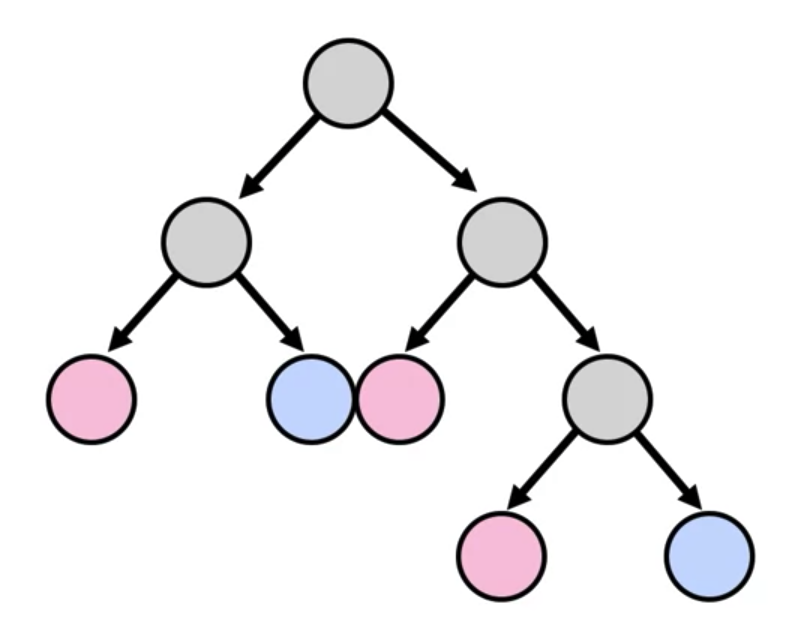
\includegraphics[scale=.5]{./figures/dectree.png}
\caption{Decision tree layout}
\label{fig1}
\end{figure}

Both regression and classification issues can be solved using decision trees. The objective is to learn basic decision rules from data attributes to develop a model that predicts the value of a target variable. They begin at the root of the tree and go via splits depending on varied outcomes until they reach a leaf node where the result is delivered.Figure~4.4 details a visual representation of the decision
tree layout.

\subsection{Bootstrapping}

The process of randomly sampling subsets of a dataset across a specified number of repetitions and variables is known as bootstrapping. To get a more accurate result, these results are averaged together.

\subsection{Random Forest Regression}

\begin{figure}[H]
\centering
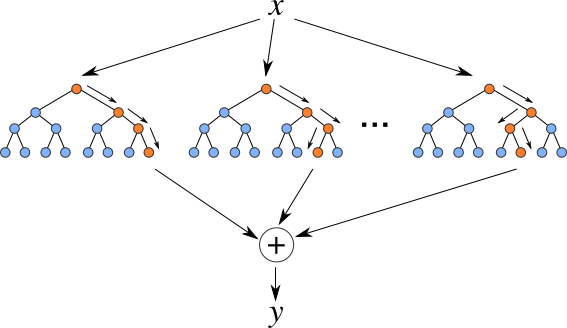
\includegraphics[width=1\textwidth, height=9cm]{./figures/rf.png}
\caption{Simple RF}
\label{fig1}
\end{figure}

The bootstrapping Random Forest algorithm \cite{B} combines ensemble learning techniques with the decision tree framework to generate numerous randomly drawn decision trees from data, then averaging the results to produce a new result that typically leads to better predictions/classifications. Figure~4.5 documents a visual
representation of random forest wherein $X$ is the feature
vector and $y$ is the target vector.

\section{MULTI LAYER PERCEPTRON}

The Multi Layer Perceptron bases its fundamental design to the
interlinking of several neuron-like structures representing a Neural
Network (NN) architecture. Given $i = 0,1,\ldots,n$ where $n$ is the
number of inputs, the quantities $w_{i}$ are the weights of the
neuron. The inputs $x_{i}$ correspond to features or variables and the
output $y$ to their prediction/estimation. Figure~4.6 shows the
simplified representation of the above steps.

\begin{figure}[h]
\centering
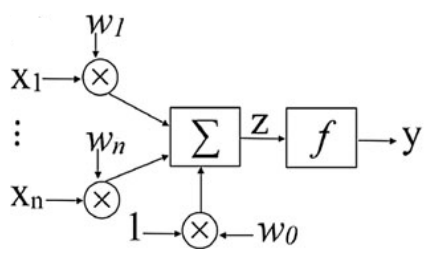
\includegraphics[]{./figures/perceptron.png}
\caption{Perceptron model}
\label{fig1}
\end{figure}

The weighting step involves the multiplication of each input feature
value by its weight ${w_ix_i}$ and then they are summed
together $(x_{0}w_{0} + x_{1}w_{1} + ... + x_{n}w_{n})$. In the transfer step, an activation function f (also called a
transfer function) is applied to the sum producing an output $y$
presented as
\begin{equation}
  z & = \sum_{i=0}^{n} w_{i}x_{i}\\
\end{equation}
\begin{equation}
  y & = f(z)
\end{equation}
wherein $x_{0} = 0$, $w_{0}$ is the bias and $y$ is the output. The
activation function can be of the form of Unit step, Linear or
Logistic operation.

For $n$
dimensions, the function is a hyperplane with equation:
\begin{equation}
    \sum_{i=0}^{n} w_{i}x_{i} = 0
\end{equation}

The goal of learning is to minimise a cost function, which is commonly a square error between the known and estimated vectors, in order to optimise the weights. The best weight vector can be determined using optimization techniques such as the gradient descent algorithm. The algorithm eventually converges on a solution that reaches an operational configuration network. The perceptron and single layer perceptron, on the other hand, do not address the nonlinearly separable problem.

\begin{figure}[h]
\centering
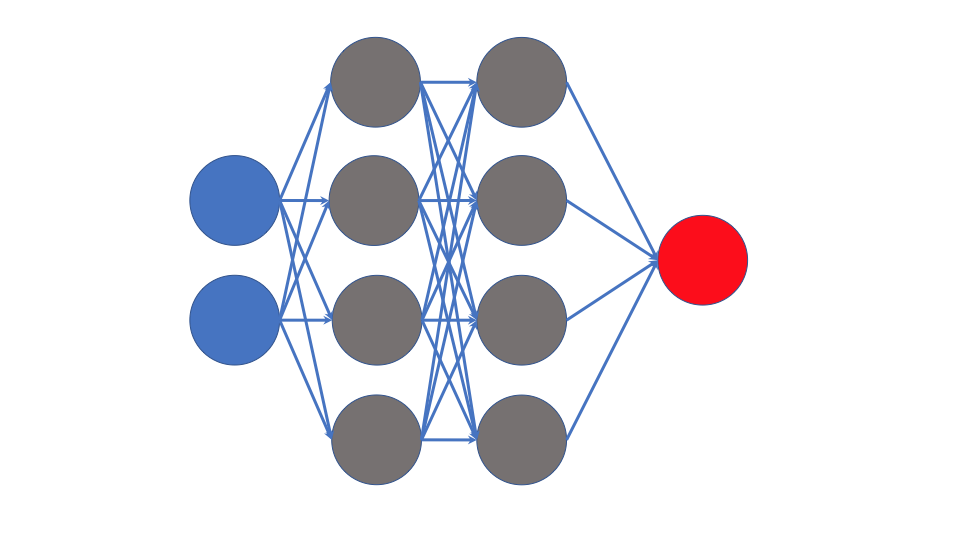
\includegraphics[width=1\textwidth]{./figures/mlp2.png}
\caption{MLP model}
\label{fig1}
\end{figure}

To solve this problem, Multi Layer Perceptron (MLP) architecture is
created by aggregating layers of perceptrons wherein the output of one
layer acts as the input of another layer. Multi Layer Perceptron
\cite{C} is a feedforward neural network that consists of three
layers, the input layer, the hidden layer and the output
layer. Figure~4.7 presents an MLP with two inputs (blue), two hidden
layers (grey) and one output (red).

The input signal to be processed is received by the input layer. The output layer is responsible for tasks such as prediction and categorization. The true computational engine of the MLP is an arbitrary number of hidden layers inserted between the input and output layers. In an MLP, data flows from input to output layer in the forward direction, similar to a feed forward network. The weights of the neurons in the MLP can be adjusted by propagating errors from layer to layer, starting with the output layer and going backwards, using the back propagation learning process. MLPs can tackle issues that aren't linearly separable and are designed to approximate any continuous function.
